\chapterbegin{Prueba de consumo}
\label{chp:consumo}
\minitoc

\sectionx{Introducci�n}
Para una exitosa implementaci�n del \ac{IOT} uno de los requisitos m�s importantes es un consumo eficiente del sistema.\\

La comunicaci�n inal�mbrica entre los nodos comienza a ser un problema cuando la fuente de alimentaci�n es limitada. Un sistema que pueda funcionar con una sola pila AAA durante a�os es lo ideal en el \ac{IOT} \cite{mahmoud2016study}. Por ello, durante el desarrollo de este proyecto se ha utilizado como protocolo inal�mbrico el IEEE 802.15.4, que destaca su bajo consumo.\\

\sectionx{Medida del consumo}

Para realizar la medida de consumo se ha utilizado el mult�metro digital Keysight 34411A, que proporciona 6 d�gitos y medio de resoluci�n y una velocidad de muestreo de 50000 muestras/s. \cite{multimeter4411A}\\

Para el control del mult�metro se ha utilizado dos programas de LabView, uno de ellos permite obtener datos a la m�xima velocidad de muestreo aunque eso limite la resoluci�n a 4 d�gitos (figura \ref{fig:capturaRapida}) y el otro programa permite tomar datos promediados en intervalos de tiempo (figura \ref{fig:capturaPromedio}).

\begin{figure}[h]
	\centering
	\begin{subfigure}[b]{0.45\textwidth}
		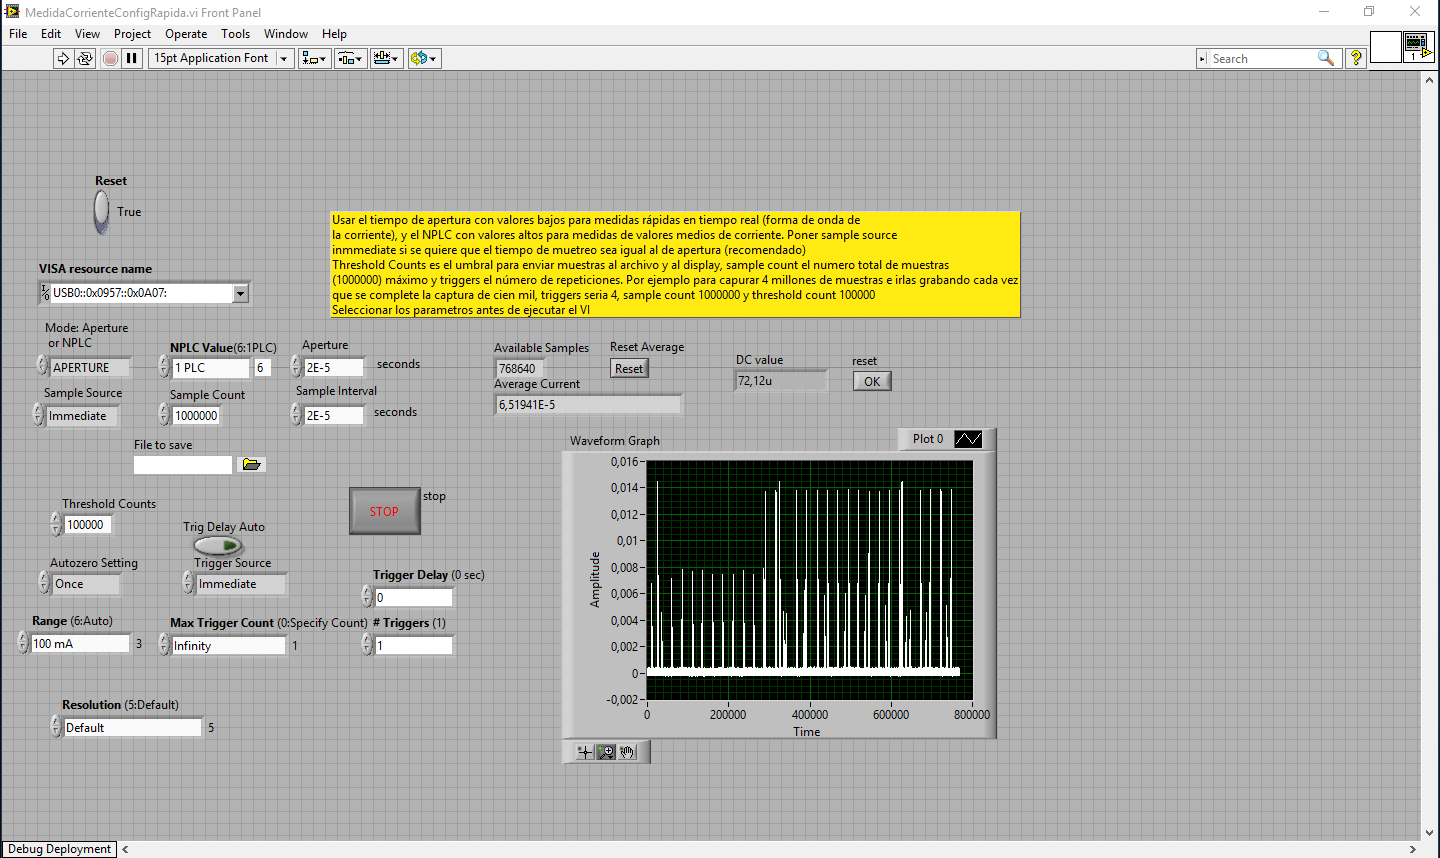
\includegraphics[width=\textwidth]{graphs/CapturaRapida.png}
		\caption{Captura r�pida}
		\label{fig:capturaRapida}
	\end{subfigure}
	\begin{subfigure}[b]{0.45\textwidth}
		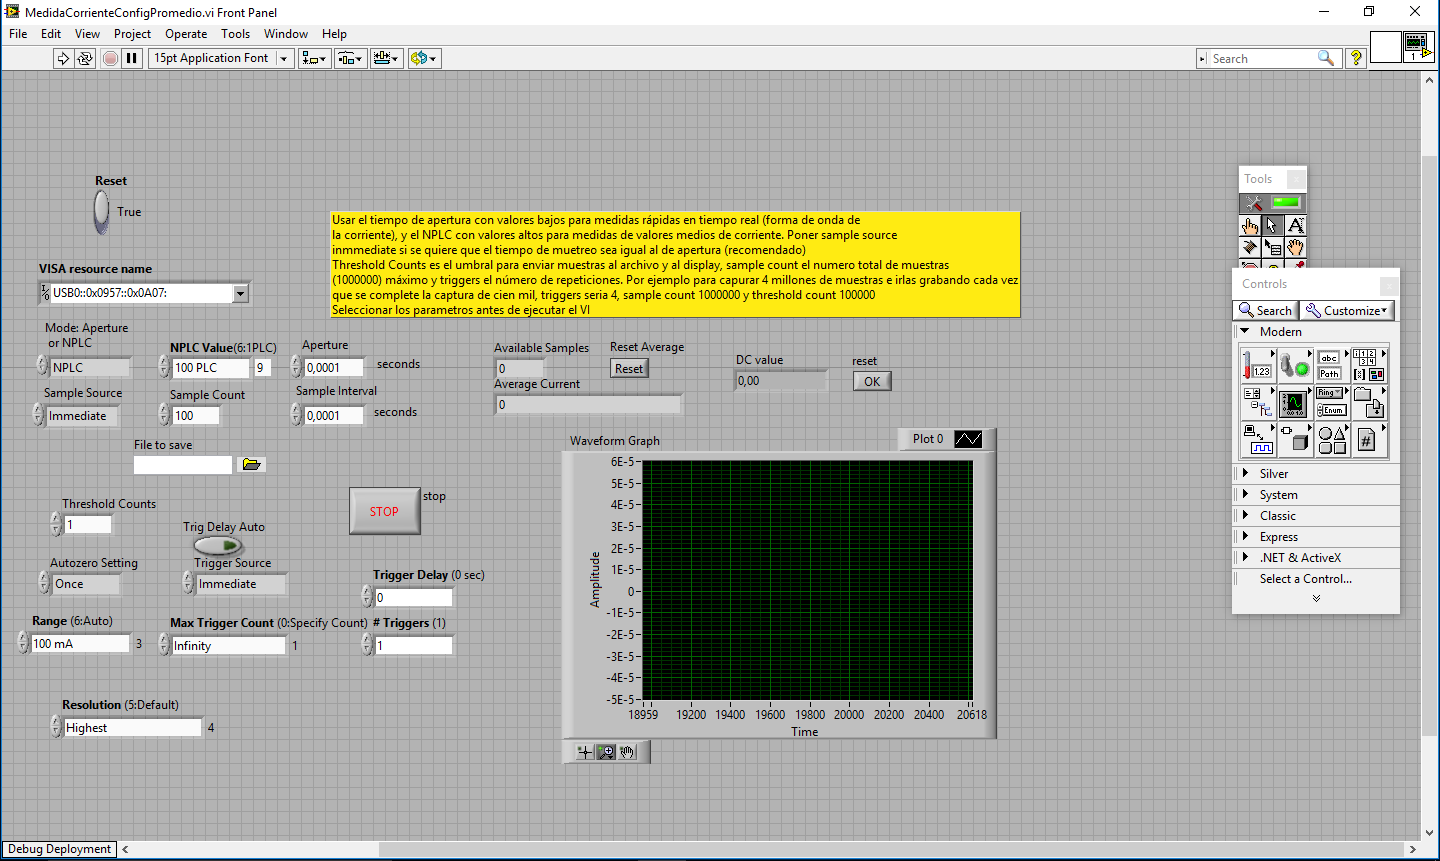
\includegraphics[width=\textwidth]{graphs/CapturaPromedio.png}
		\caption{Captura promedio}
		\label{fig:capturaPromedio}
	\end{subfigure}
	\caption{Programas de LabView}
	\label{fig:capturasLabview}
\end{figure}

\sectionx{Resultados}

Aunque el objetivo de esta prueba es conocer el consumo medio de corriente del nodo. Antes de nada se necesita conocer que fondo de escala utilizar en el mult�metro para la medida en promedio, para ello se hace uso del programa de captura a m�xima frecuencia de muestreo, donde se obtiene la corriente instant�nea m�xima que consume el nodo, unos 15 mA (figura \ref{fig:datosCapturaRapida}).

\begin{figure}[h]
	\centering
	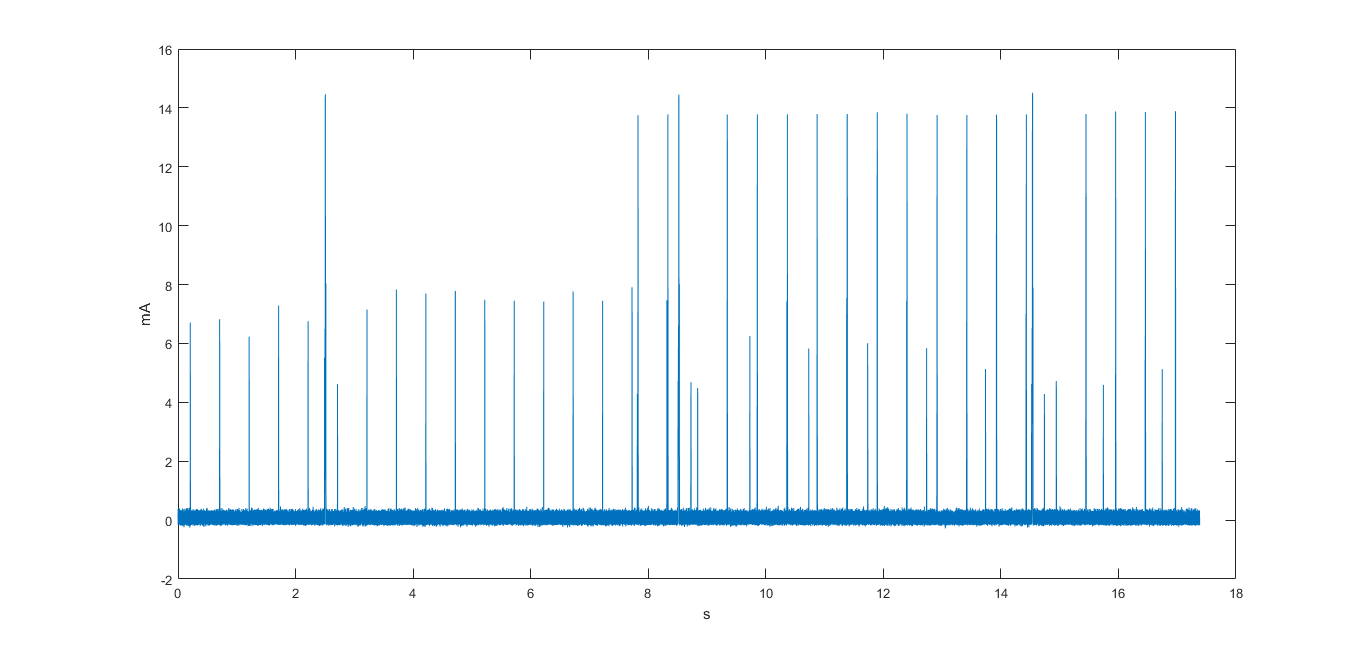
\includegraphics[width=0.8\textwidth]{graphs/capturaRapidaDatos.png}
	\caption{Consumo en mA del nodo a la m�xima frecuencia de muestreo}
	\label{fig:datosCapturaRapida}
\end{figure}

Finalmente, utilizando el programa de medida promediada de LabView con un fondo de escala de 100mA, realizamos una medida de la corriente promedio durante 50 ciclos de subidas al servidor. Con esta configuraci�n se obtiene que el consumo medio de un nodo es de 169.6 $\micro A$, lo que equivale a m�s de 5 meses de funcionamiento utilizando una pila de bot�n CR 2477. 


\chapterend{}